\documentclass[10pt, compress]{beamer}

\usetheme{metropolis}
\usepackage{appendixnumberbeamer}

\usepackage{tikz-dependency}
\usepackage{caption}
\usepackage{booktabs}
\usepackage[scale=2]{ccicons}

\usepackage{pgfplots}
\usepgfplotslibrary{dateplot}

\usepackage{xspace}
\newcommand{\themename}{\textbf{\textsc{metropolis}}\xspace}

% commands from the paper
\newfontfamily\gtfont[Scale=1.1,Letters=SmallCaps]{Linux Libertine O}
\newcommand{\udtag}[1]{{\ll \textsc{#1}}}
\newcommand{\gtlabel}[1]{{\gtfont #1}}
\newcommand{\udlabel}[1]{{\tt #1}}
\newfontfamily\udfont[Scale=0.9,Letters=SmallCaps]{Linux Libertine O}
\newcommand{\utag}[1]{{\udfont#1}}
\newcommand{\ufeat}[1]{{\udfont#1}}
\newcommand{\tgl}[1]{{\em #1}}
% commands from the paper


\newcommand{\myarrow}[1][-45]{%
  \mathrel{%
    \text{$
     \begin{tikzpicture}[baseline = -0.5ex]
       \node[inner sep=0pt,outer sep=0pt,rotate = #1] (a) at (0,0)  {$\xrightarrow{}$};
    \end{tikzpicture}
    $}%
  }%
}%




\title{Class 01: Getting started }

\begin{document}

\maketitle

\begin{frame}{Why are you taking this course?}

\end{frame}

\begin{frame}{Structure of the course}

\begin{center}
\begin{tabular}{rlrl}
1  &  & 7   & \emph{Project work}  \\
2  &  & 8   &  \emph{Project work} \\
3  &  & 9   &  \emph{Project work} \\
4  &  & 10   &  \emph{Project work} \\
5  &  & 11   & \emph{Project work}  \\
6  &  & 12   & \emph{Presentations}  \\
\end{tabular}
\end{center}

\end{frame}

\begin{frame}{Prerequisites}

Stuff you need before you begin:
\begin{itemize}
 \item A UNIX-compatible system (GNU/Linux, *BSD, Mac/OS)
 \item A text editor
 \item An installation of Python -- Python 3.0 or higher!
\end{itemize}

How to choose a text editor:

\begin{center}
  
\includegraphics[width=0.6\textwidth]{graphics/realprogrammers.png}
\end{center}

Honestly, use something other people (programmers) you know use.

\end{frame}

\begin{frame}{How to get help}

\begin{center}
  \begin{onlyenv}<1>
  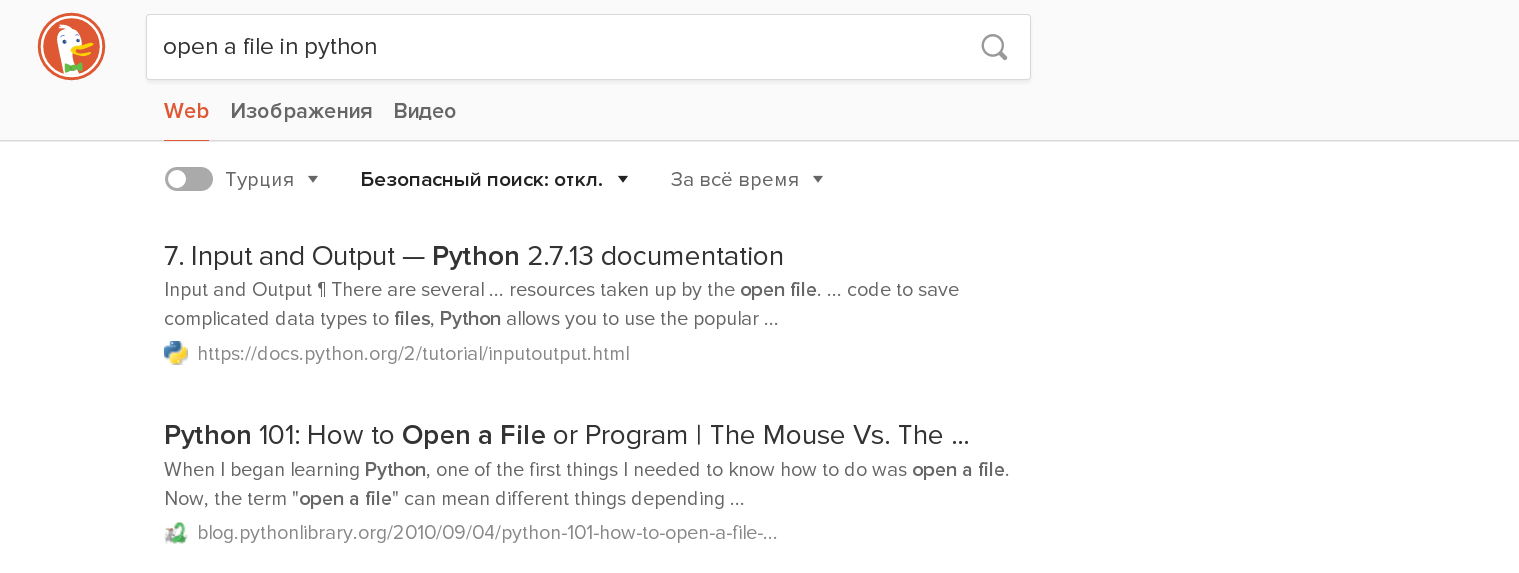
\includegraphics[width=0.6\textwidth]{graphics/duckduckopenfile.png}
  \end{onlyenv}
  \begin{onlyenv}<2>
  
\includegraphics[width=0.6\textwidth]{graphics/pythondocs.png}
  \end{onlyenv}
  \begin{onlyenv}<3>
  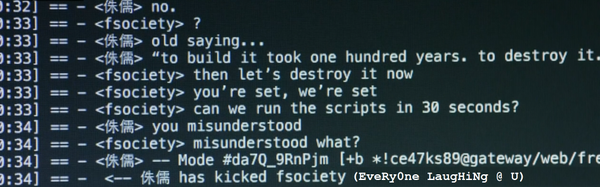
\includegraphics[width=0.6\textwidth]{graphics/CKmO8DXVAAAWl1d.png}
  \end{onlyenv}
\end{center}

On your own:
\begin{itemize}
  \item A search engine such as Google™, Yandex™ or DuckDuckGo™
  \item The fine Python documentation at \url{http://docs.python.org}
  \item Internet Relay Chat
  \item Stack Overflow
\end{itemize}

Ask me:
\begin{itemize}
  \item In class
  \item Outside class: IRC, VK, Google Hangouts
\end{itemize}

\end{frame}

\begin{frame}{What we are going to do today}

First things first:
\begin{itemize}
  \item Make sure you have Python installed
  \item Set up Github accounts
  \item Install a text editor
\end{itemize}

Then second things:
\begin{itemize}
  \item Choose a language
  \item Download the Wikipedia in that language 
  \item Extract the text from Wikipedia
\end{itemize}

\end{frame}

\begin{frame}{Github}

\end{frame}

\begin{frame}{Text editor}

% Sublime: +
% Vim:
% Emacs:


\end{frame}

\begin{frame}{Wikipedia as a corpus/1}

\begin{center}
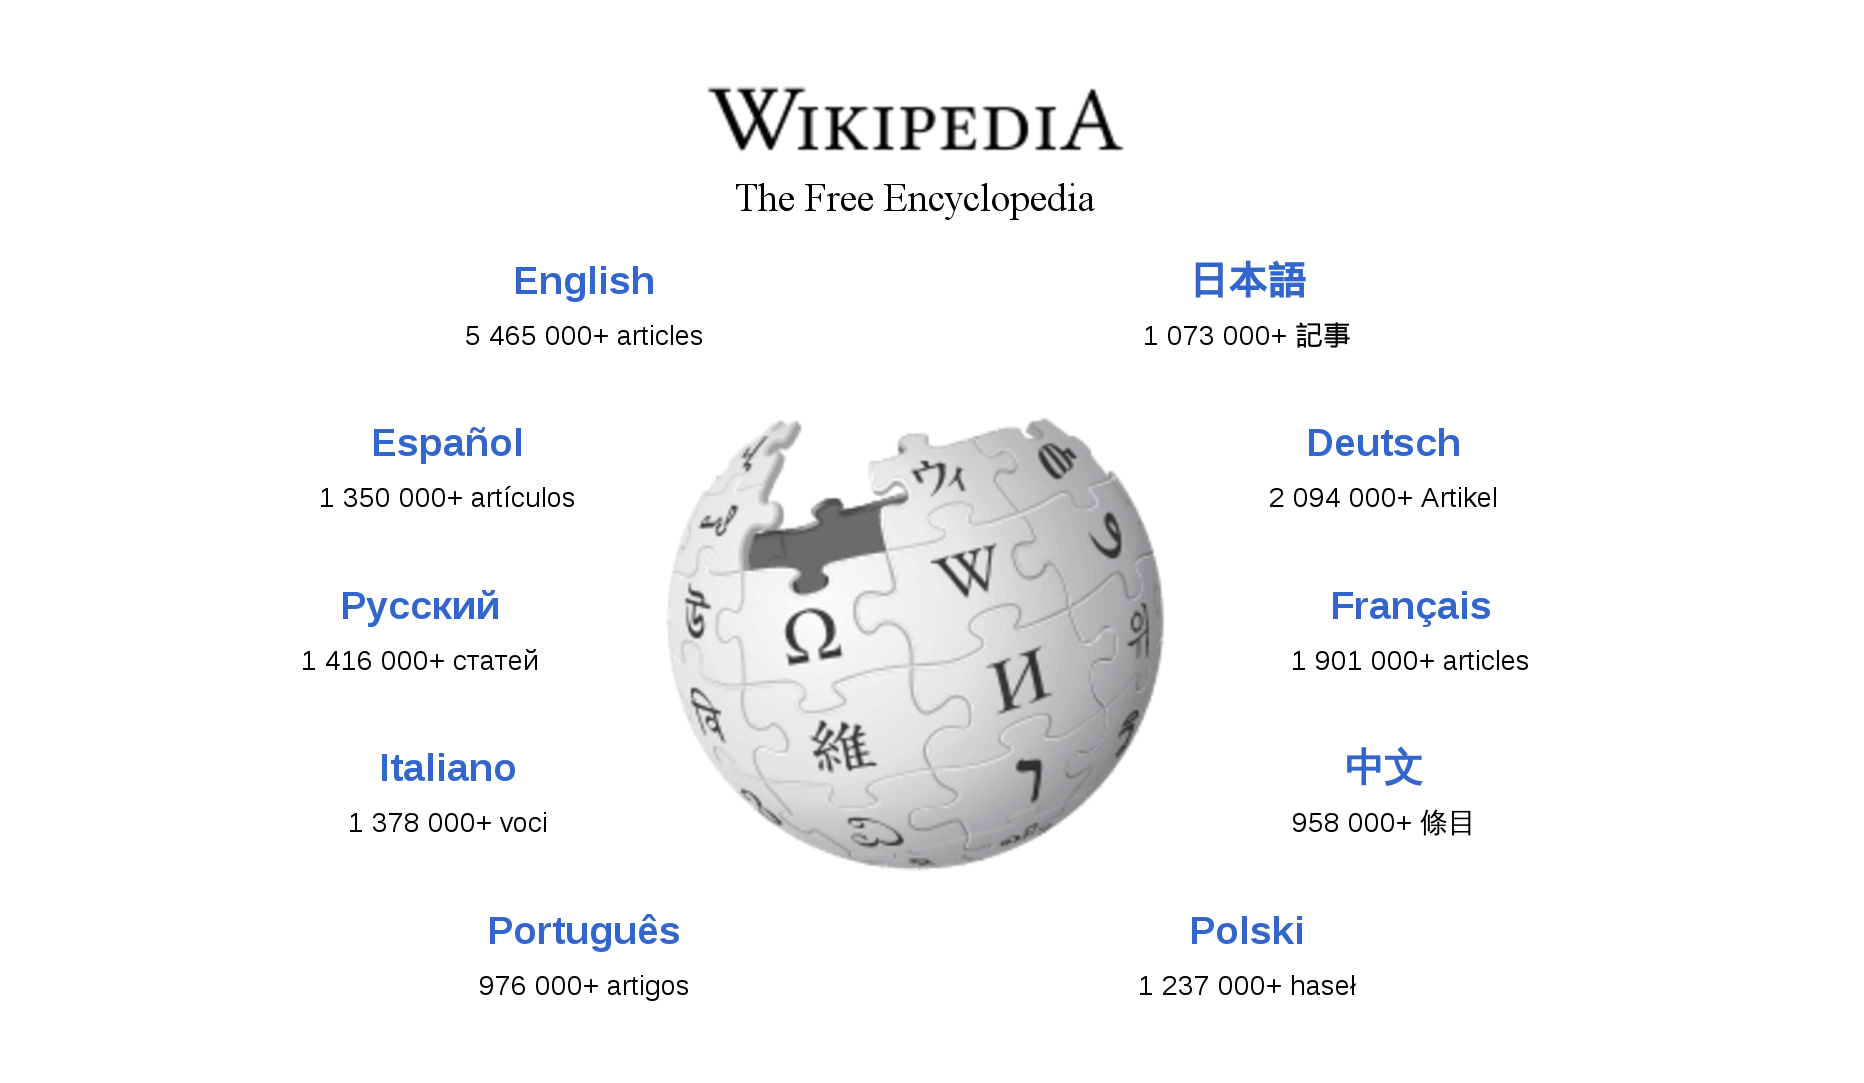
\includegraphics[width=0.70\textwidth]{graphics/wikipedia-front.png}
\end{center}

Wikipedia makes a great\footnote{Well, great in some respects} corpus:

\begin{itemize}
   \item Free to use and distribute
   \item Very many languages -- 295 at the last count
\end{itemize}

\end{frame}

\begin{frame}{Wikipedia as a corpus/2}

Deliberately vague steps:

\begin{itemize}
  \item Use your search engine to find where Wikipedia keeps it's `dumps'.
  \item Find the language code of the language you are interested in
  \item Download the dump for the language you are interested in
  \begin{itemize}
    \item Tip 1: You're looking for a `Database backup dump'
    \item Tip 2: The filename will include {\tt pages-articles.xml.bz2}
  \end{itemize}
  \item Find WikiExtractor on the Apertium Wiki
  \item Run WikiExtractor on the dump file you downloaded. 
\end{itemize}

\end{frame}





\end{document}

